\section{Modifier les sources de paquets}\subsection{Information}
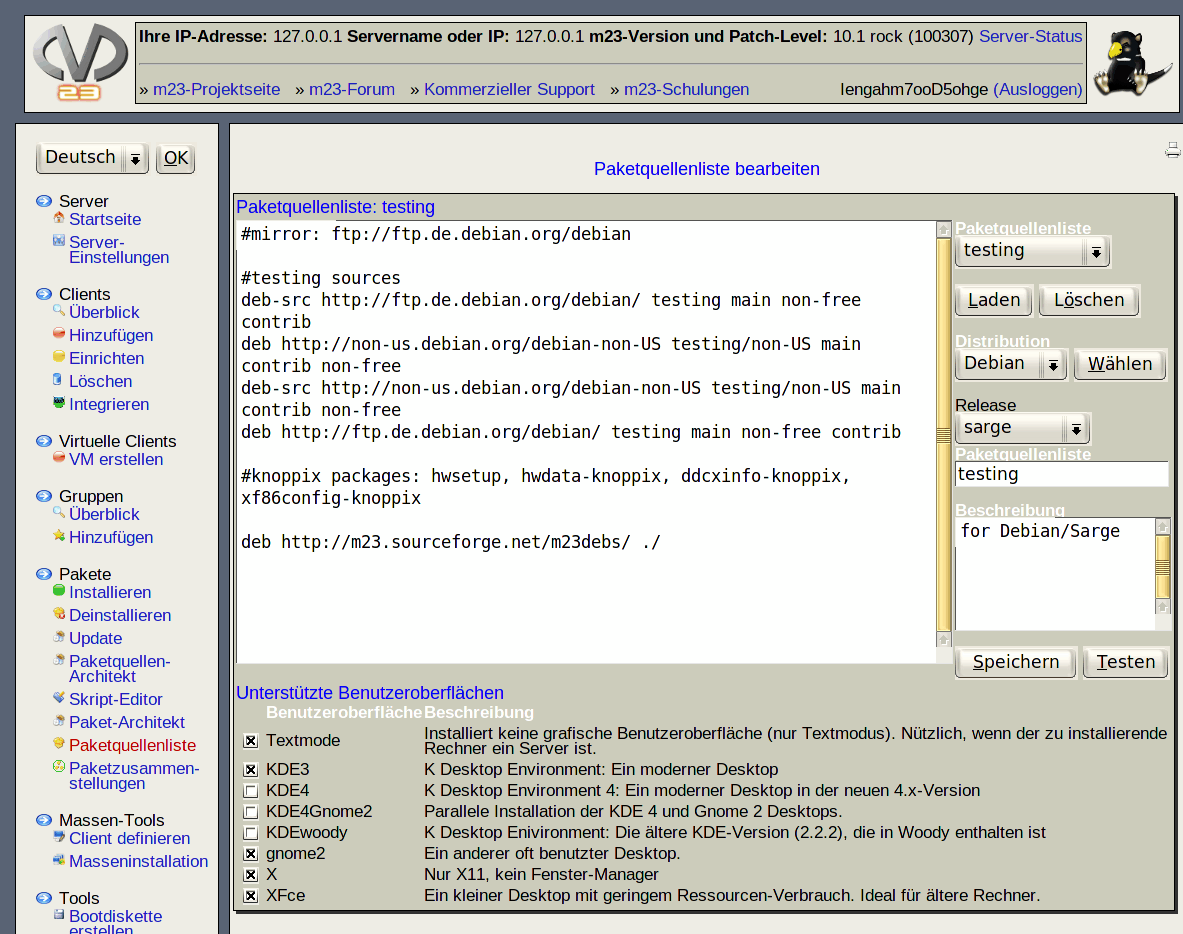
\includegraphics[scale=0.4]{/mdk/doc/manual/screenshots/fr/client_sourceslist.png} \\
Des paquets de logiciel peuvent \^etre install\'e \`a partir de diff\'erentes sources (HTTP,FTP,CDRom etc.). Des sources diff\'erentes deviennent n\'ecessaires, quand on ne peut pas installer tous les paquets de logiciel d'un medium singulier. Pour vous donner une possibilit\'e simple d'administrer les sources, vous les entrez comme vous l'\^etes habitu\'e de la distribution choisie.\\
\begin{itemize}
	\item \textbf{Charger une source de paquets}: Pour le chargement, vous choisissez la source de paquets que vous voudriez charger de la liste en haut. Apr�s un clic sur \textit{$\ll$Charger$\gg$}, elle sera charg� dans l'�diteur.\\
	\item  \textbf{Effacer une source de paquets}: Pour effacer la source de paquets charg� dans l'�diteur, cliquez sur le bouton \textit{$\ll$Effacer$\gg$} et consentiez � l'effacement au dialogue suivant.\\
	\item  \textbf{Enregistrer une source de paquets}: Il sera toujours enregistr� la source de paquets charg�e dans l'�diteur, ind�pendant de celle qui est montr�e dans la liste en haut. D'abord, choisissez la distribution � laquelle la liste des paquets doit s'appliquer. Apr�s que vous auriez choisi la distribution, il se peut passer que vous devez entrer des valeurs suppl�mentaires. En plus, s�lectionnez les interfaces graphiques support�s de la liste des sources de paquets de la liste sous la case de l'�diteur.  Trouvez un nom pour la liste de paquets et entrez-le dans le champ de saisie sous \textit{$\ll$Nom de source de paquets$\gg$}. Si vous avez charg� une source de paquets, le nom sera entr�e automatiquement. Si vous voulez, vous pouvez entrer un commentaire dans le champ \textit{$\ll$Description$\gg$}. Puis, cliquez sur \textit{$\ll$Enregistrer$\gg$}.\\
	\item  \textbf{Tester une source de paquets}: Apr�s avoir entr�e une source de paquets, vous devriez essayer si elle fonctionne conform�ment � l'ordre. Apr�s un clic sur le bouton \textit{$\ll$Tester$\gg$}, le programme essaie de t�l�charger les d�scriptions des paquets des sources. Apr�s l'ach�vement de l'essai un rapport du teste sera montr�. Il peut prendre quelques minutes jusqu'� ce que le rapport du teste apparaisse. La vitesse d�pend de votre connection � l'internet et de la vitesse des serveurs de sources de paquets utilis�s.\\
        \item \textbf{Entrer le site miroir}: Si vous voudriez utiliser un site miroir diff�rent (le site miroir de standard est ftp.debian.org) pour l'installation du syst�me de base, entrez-le dans une nouvelle ligne dans la source de paquets comme c'est d�crit au suivant: \\
\begin{verbatim}
#mirror: [URL des paquets]
\end{verbatim}
. \textit{URL des paquets} signifie le protocole, le nom d'h�te ou l'adresse IP et le r�pertoire, o� les paquets peuvent �tre trouv�s. Une ligne valide pourrait se pr�senter comme au suivant, par exemple: \\
\begin{verbatim}
#mirror: http://192.168.7.14/debianCDs
\end{verbatim}
\end{itemize}
\subsection{Information suppl\'ementaire}
\begin{itemize}
\item Si vous enregistrez une source de paquets sous un nom existant, la vieille source de paquets sera remplac\'ee.\\
\item Les \textbf{interfaces graphiques} d\'ependent directement d'une liste de sources de paquets. �a veut dire que vous pouvez uniquement utiliser les interfaces graphiques que vous avez choisis dans ce dialogue pour la liste des sources de paquets que vous voudriez utiliser pour un certain poste client. Pour cette raison, vous devriez seulement choisir les interfaces graphiques ici qui sont vraiment support\'es des sources de paquets.\\
\end{itemize}
